\section{The ZFOURGE Survey} \label{Sec: The ZFOURGE Survey}
\subsection{Overview}

This study utilises the 2017 release\footnote{Available for download at \href{https://zfourge.tamu.edu/}{zfourge.tamu.edu.}} of the ZFOURGE survey \citep{straatman_fourstar_2016}, which offers a unique combination of depth and wavelength coverage essential for probing high-redshift galaxies and constructing accurate LFs. ZFOURGE consists of approximately 70,000 galaxies at redshifts greater than 0.1, covering three major 11$\times$11 arcminute fields: the Chandra Deep Field South (CDFS) \citep{giacconi_chandra_2002}, the field observed by the Cosmic Evolution Survey (COSMOS) \citep{scoville_cosmic_2007}, and the CANDELS Ultra Deep Survey (UDS) \citep{lawrence_ukirt_2007}. These galaxies were observed using the near-infrared FourStar imager \citep{persson_fourstar_2013} mounted on the 6.5-m Magellan Baade Telescope at the Las Campanas Observatory in Chile.  

ZFOURGE employs deep near-infrared imaging with multiple medium-band filters (\textit{J}$_{1}$, \textit{J}$_2$, \textit{J}$_{3}$, \textit{H}$_{l}$, \textit{H}$_{s}$) and a broad-band \textit{K}$_{s}$ filter. The imaging spans 1.0 to 1.8 $\mu$m and achieves 5$\sigma$ point-source limiting depths of 26 AB mag in the \textit{J} medium-bands and 25 AB mag in the \textit{H} and \textit{K}$_{s}$ bands \citep{spitler_first_2012}. These filters yield well-constrained photometric redshifts, particularly effective for sources within the redshift range of 1 to 4 \citep{spitler_first_2012}. ZFOURGE data is supplemented by public data from HST/WFC3 F160W and F125W imaging from the CANDELS survey, Spitzer/Infrared Array Camera (IRAC), and Herschel/Photodetector Array Camera and Spectrometer (PACS). For a detailed description of the data and methodology, refer to \cite{straatman_fourstar_2016}.

\subsection{Sample Selection} \label{Sec: Sample Selection}
\subsubsection{ZFOURGE Sample} \label{Sec: Galaxy LF Selection}
ZFOURGE is a near-infrared-selected survey and, as such, may be biased against the most heavily dust-obscured galaxies, particularly at higher redshifts where the observed near-IR corresponds to rest-frame optical or ultraviolet wavelengths. This limitation is well established in the literature (e.g., \citealp{fu_decomposing_2010, grazian_galaxy_2015}) and is an inherent selection effect of deep near-IR surveys. As a result, the sample may underrepresent certain populations of extremely obscured star-forming galaxies and AGN. Nonetheless, the dataset includes a substantial number of dusty sources across all fields (e.g., \citealp{spitler_exploring_2014}), and many highly obscured systems, particularly those with high intrinsic luminosities, are still likely to be included due to their brightness in mid-IR or even near-IR bands (e.g., MIPS 24$\mu m$). 

To ensure the selection of high-quality galaxies and minimise errors in our analysis, we adopt the ZFOURGE quality flag \texttt{Use=1}, as defined by \cite{straatman_fourstar_2016}. This flag selects galaxies with reliable photometry and redshift measurements, resulting in a starting sample of 37,647 galaxies.

To ensure a physically meaningful sample, we excluded sources with negative infrared luminosities (LIR) derived from the \cite{wuyts_fireworks_2008} template fitting. These negative values arise from noise-dominated fluxes, particularly at 24–160$\mu m$, where photometric fluctuations result in unphysical luminosity estimates. Their removal introduces a minor level of incompleteness, but does not impact the reliability of the luminosity functions in the well-sampled, physically meaningful regime. After excluding galaxies with unphysical total IR luminosities ($L_{IR} < 0$), the sample is reduced to 22,997 galaxies. 

We apply a redshift cut, restricting the sample to $0 \leq z \leq 6$ since only 28 galaxies exist at $z > 6$ (yielding  22,967 galaxies). This redshift range enables us to observe the evolution of galaxies during some of the most critical cosmic periods, specifically around $1 < z < 3$ \citep{gruppioni_modelling_2011, wylezalek_galaxy_2014} where galaxy luminosity density peaks \citep{assef_mid-ir-_2011}.

To ensure robustness, we calculate the estimated total IR flux in each sample using the luminosity-distance equation and apply an 80\% completeness flux cut. Refer to section \ref{Sec: IR_Luminosity} for a description on how the total IR luminosities were derived. This reduces the impact of noise and observational limits while preserving a large enough sample for LF construction. The final ZFOURGE sample includes 18,373 galaxies.

\subsubsection{Decomposed Samples} \label{Sec: Decomposed AGN Selection}
The ZFOURGE survey is first decomposed into SF and AGN components using the CIGALE software. Each ZFOURGE source has a component AGN and SF luminosity in the CIGALE samples. For a comprehensive explanation of the SED decomposition process, please refer to Section \ref{Sec: CIGALE}. We continue to apply the ZFOURGE survey's \texttt{Use=1} for our analysis, resulting in an initial sample of 37,647 sources for both the AGN and SF samples. Most objects will have a variable combination of AGN and SF that fit into both decomposed samples. We do not remove ZFOURGE sources labelled $L_{IR}<0$ in the SF or AGN samples and instead let CIGALE recalculate the component luminosities. As such, the decomposed samples may have more sources than the ZFOURGE sample. 

For our AGN-specific analysis, we include all sources with a significant AGN fraction ($\mathcal{F}_{AGN}>0.1\ L_{AGN}/L_{IR}$); 21,063 sources. We apply an 80\% total IR flux cut (calculated from the total SF and AGN luminosities, respectively) to both decomposed samples as was performed with ZFOURGE. After applying each flux cut, the SF and AGN sample is reduced to a final set of 16,850 and 30,059 sources, respectively, spanning $0 \leq z \leq 6$. 

Throughout this work, we use ``decomposed" to refer to the CIGALE SF and AGN luminosities and samples and ``ZFOURGE" to refer to the original ZFOURGE luminosities and dataset. To avoid confusion, the ``total luminosities” referred to in this work are infrared luminosities integrated over rest-frame 8–1000$\mu$m, and do not include emission from X-ray, UV, or radio wavelengths.

Figure \ref{Fig: ZF Lum vs z} shows the reduced luminosity-redshift distribution of ZFOURGE (top), CIGALE AGN (middle), and CIGALE SF (bottom). The jagged boundaries between redshift bins represent the luminosity completeness limit of the respective luminosity function. The luminosity completeness limit is defined as the turnover in the luminosity function.

\begin{figure}
    \centering
    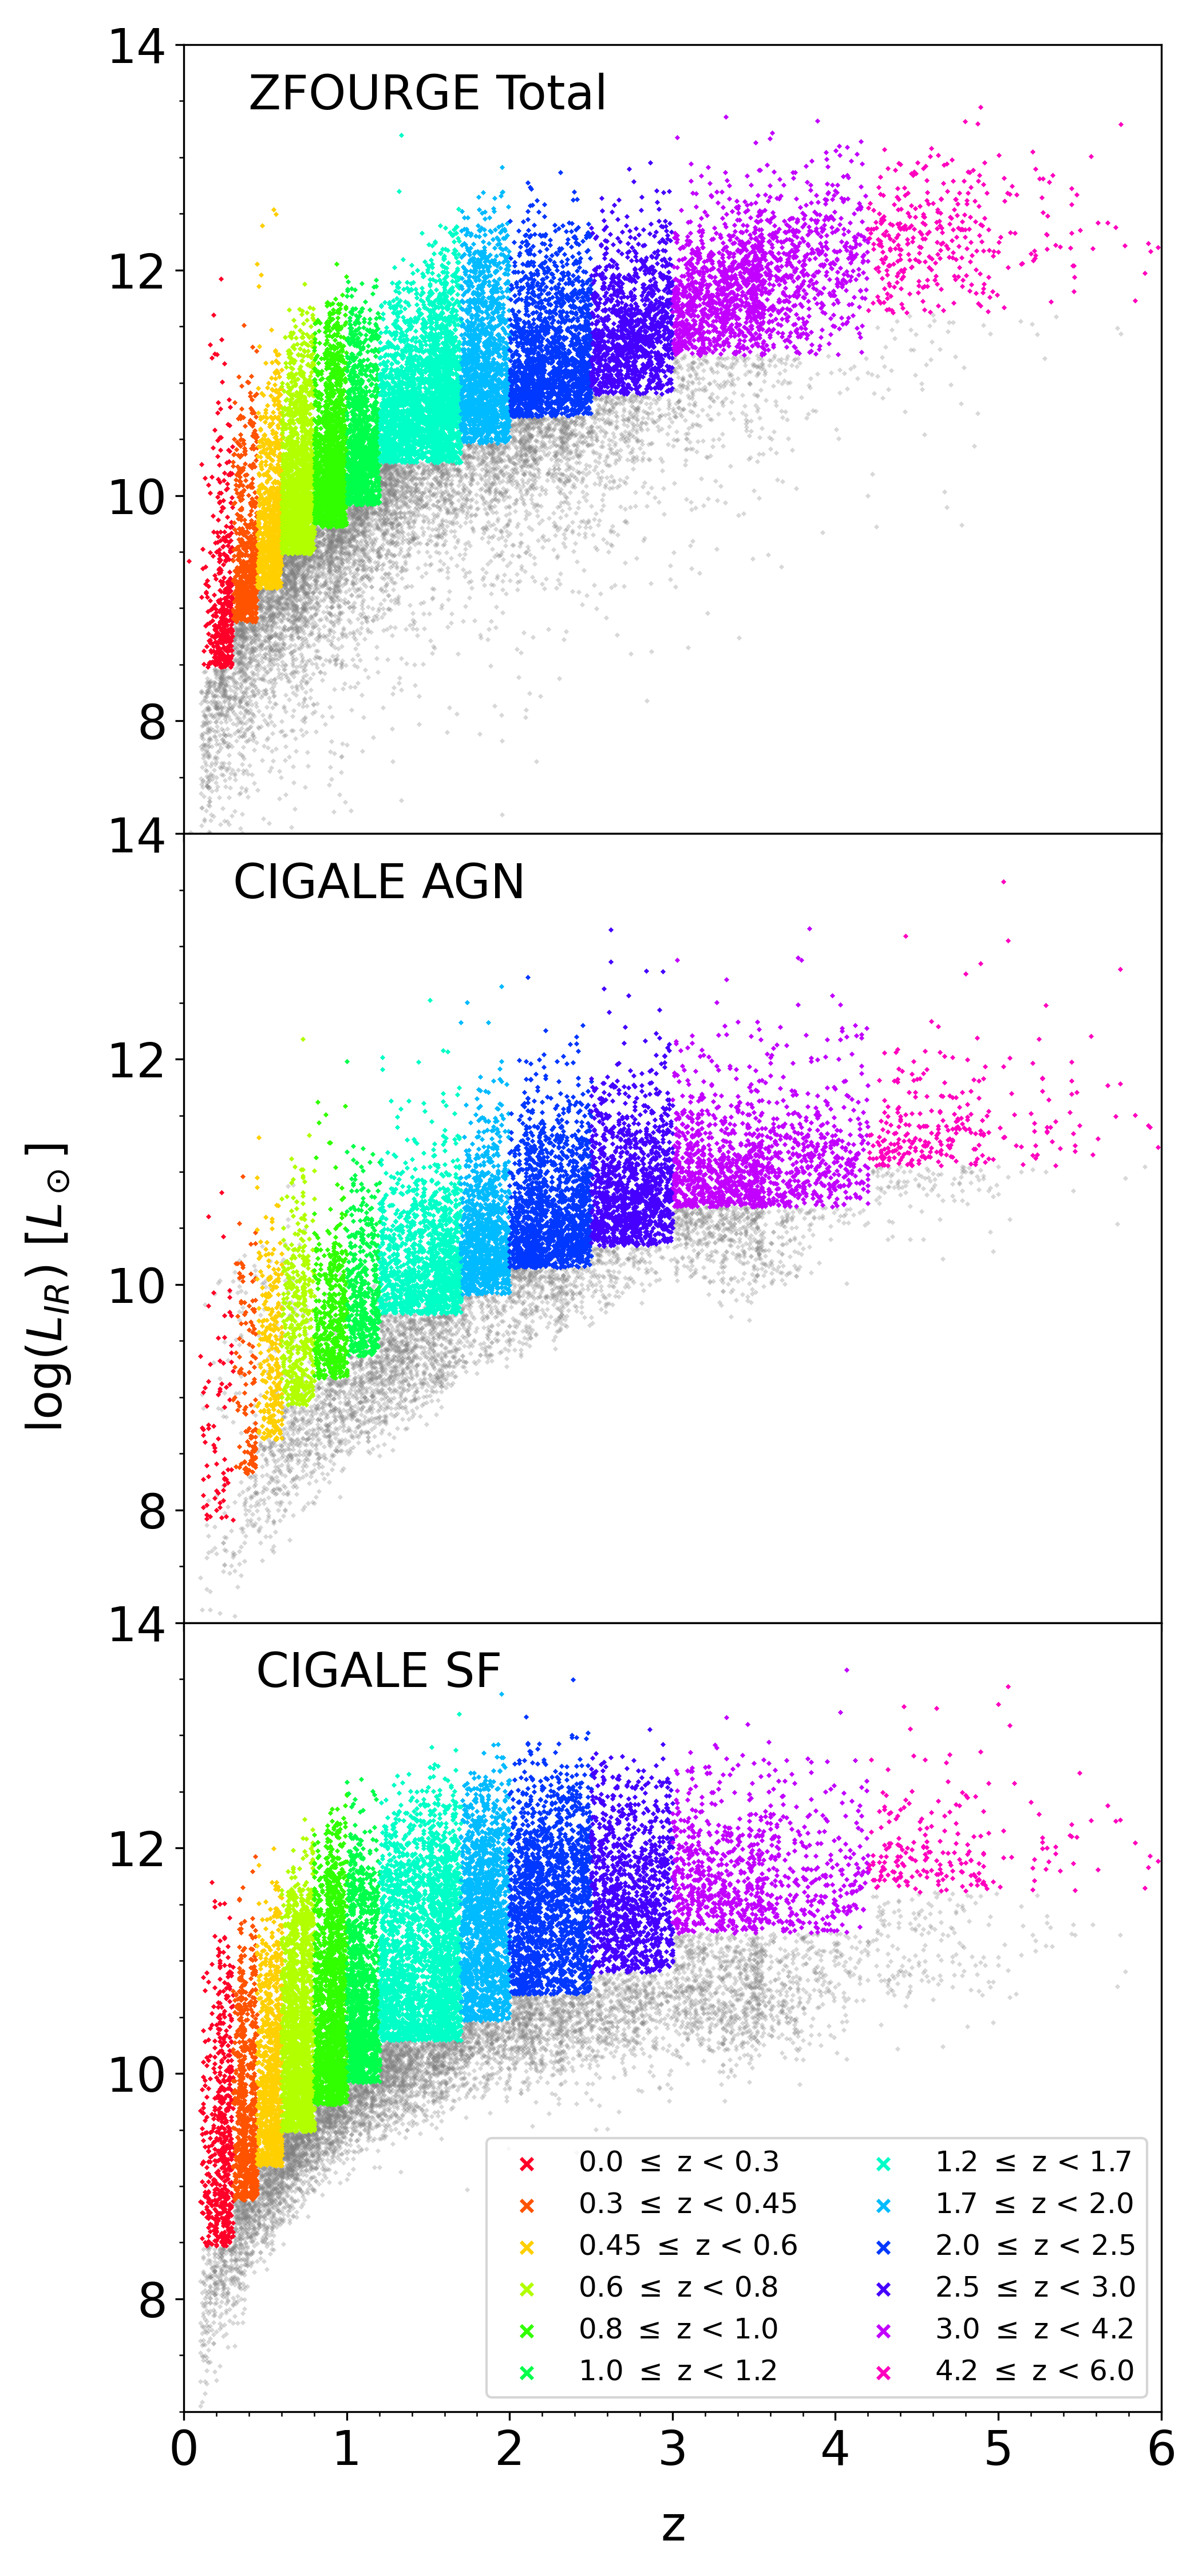
\includegraphics[width=0.7\textwidth]{Figures/LIR_vs_Z.png}
    \caption{Luminosity-redshift distributions of (top) the ZFOURGE $8-1000\mu m$ luminosity, (middle) the CIGALE AGN luminosity, and (bottom) the CIGALE SF luminosity. Sources are coloured by redshift bin or coloured grey if removed as described in section \ref{Sec: Sample Selection}}
    \label{Fig: ZF Lum vs z}
\end{figure}













\section{Decomposing Galaxy SEDs} \label{Sec: CIGALE}
The public version of the ZFOURGE catalogues has utilised \texttt{EAZY} \citep{brammer_eazy_2008} and \texttt{FAST} \citep{kriek_ultra-deep_2009} for parameterising galaxy properties, primarily focusing on photometric redshifts, stellar masses, and SFRs. However, while effective, these methods provide a more generalised view of galaxy properties without entirely disentangling the contributions from different physical components within each galaxy, such as SF regions and AGN. To address this limitation, we employ the SED fitting software CIGALE \citep{boquien_cigale_2019}, which enables the decomposition of observed light from galaxies into distinct components, including SF and AGN activity. This method builds on the work by \cite{cowley_decoupled_2018}, incorporating additional photometric coverage and an updated parameter space to better quantify AGN contributions.

\subsection{CIGALE Methodology and Parameter Space} \label{Sec: CIGALE_Parameters}
CIGALE performs multi-component SED fitting to derive galaxy properties by integrating our photometry from 0.2 $\mu$m to 160 $\mu$m across the CDFS field and up to 24 $\mu$m for COSMOS and UDS. This broader wavelength coverage allows for a more complete and precise decomposition of galaxy light into SF and AGN components. The decomposition uses a range of parameter values (see Table \ref{tab:parameter_space}), allowing for flexible modelling of star formation histories (SFH), dust attenuation, AGN torus contributions, and other factors. We also incorporate the SKIRTOR AGN torus model \citep{stalevski_dust_2016}, which better handles clumpy dust distributions and polar dust extinction, providing an accurate characterisation of AGN emission.

The ZFOURGE sample has the following photometry: IRAC 3.6$\mu m$ (S/N $\geq$ 1): 98.84\%; MIPS 24$\mu m$ (S/N $\geq$ 1): 69.09\%; and Herschel PACS 70-160$\mu m$ (S/N $\geq$ 1): 11.84\%. With each band increasing to 99.47\%, 100\% and 26.19\% at S/N $\geq$ 0 respectively. 

\subsection{Total IR Luminosity Derivation} \label{Sec: IR_Luminosity}
Understanding the total IR energy output of galaxies is essential for tracing both SF and AGN activity, particularly in dusty environments where much of the energy is re-emitted in the IR \citep{fu_decomposing_2010}. By estimating the total IR luminosity, we can gain insights into the contribution of these processes across cosmic time. 

For the ZFOURGE LF sample, we adopted the approach in \cite{straatman_fourstar_2016} where the averaged \cite{wuyts_fireworks_2008} template was fit to the 24-160 $\mu$m photometry to estimate the total IR luminosity. However, at $z>3$, we find an offset of 0.27 dex in ZFOURGE luminosity over CIGALE luminosity. This is readily seen in Figure \ref{Fig: LIR vs LIR} (top) as the purple/magenta dots. These sources are also highly AGN-dominated. Because \cite{wuyts_fireworks_2008} only samples the 24-160$\mu m$ range, in conjunction with our dataset hosting only a small fraction of FIR data, our ZFOURGE luminosities at $z>3$ are likely overestimated. To account for this, we add in quadrature to the ZFOURGE $L_{IR}$ an error of 0.27 dex in addition to $z_{phot}$ and $L_{IR}$ errors.

For the CIGALE decomposed SF and AGN LF samples, we derive luminosities through a different approach. CIGALE performs SED decomposition on the entire galaxy emission, using its integrated models to separate the total luminosity into distinct stellar, dust, and AGN components. The stellar and dust luminosities are combined to form the SF component, while the AGN component is derived directly from CIGALE's emission modelling. These distinct approaches are subsequently used to construct the IR luminosity functions of the two samples. 

Figure \ref{Fig: LIR vs LIR} compares the CIGALE decomposed total luminosity to the ZFOURGE total luminosity ($L_{IR}$). In the top panel, galaxies are coloured based on their redshift bin. It can be seen that the brightest galaxies are more likely to exist at higher redshifts. In the bottom panel, galaxies are coloured based on the AGN fraction ($\mathrm{F}_{AGN}$) to the total luminosity derived by CIGALE. Galaxies at higher redshift are brighter and more likely to host a powerful AGN. At higher redshifts, there is more gas available to fuel powerful SF and AGN activity. This reflects a period of intense growth seen in the early universe \citep{madau_cosmic_2014}.

\begin{table}[htbp]
    \caption{Parameter space used for SED fitting with CIGALE}
    \label{tab:parameter_space}
    \begin{center}
    \begin{tabular}{ll}
        \toprule
        \textbf{Parameter} & \textbf{Model/Values} \\ 
        \hline
        SFH                 & Delayed SFH $\tau = 1,3,5,7,9,11$ Gyr \\
        Age                 & $0.5, 1, 3, 5, 7, 9, 11$ Gyr \\
        Burst Fraction      & $0.0, 0.01, 0.05, 0.1, 0.15, 0.2, 0.3$ \\
        SSP                 & \cite{bruzual_stellar_2003} \\
        IMF                 & \cite{chabrier_galactic_2003} \\
        Metallicity         & Fixed at 0.02 \\
        Nebular             & \cite{inoue_rest-frame_2011} \\
        Dust Atten.         & \cite{calzetti_dust_2000} $E_{(B-V)} = 0.01, 0.05, 0.1, 0.5$, \\
                            & $1.0, 1.5$ \\
        Dust Emission       & \cite{dale_two-parameter_2014} $\alpha = 1.0, 1.5, 2.0, 2.5, 3.0$ \\
        AGN Model           & SKIRTOR \citep{stalevski_3d_2012, stalevski_dust_2016} \\
        Torus Inclination   & $30^\circ, 70^\circ$ \\
        AGN Fraction        & $0.0, 0.01, 0.1 - 0.9$ (steps of 0.1), 0.99 \\
        Polar Extinction    & SMC $E(B-V) = 0.0, 0.03, 0.1, 0.2, 0.4, 0.6, 1.0, 1.8$ \\
        \bottomrule
    \end{tabular}
    \end{center}
\end{table}

\begin{figure}
    \centering
    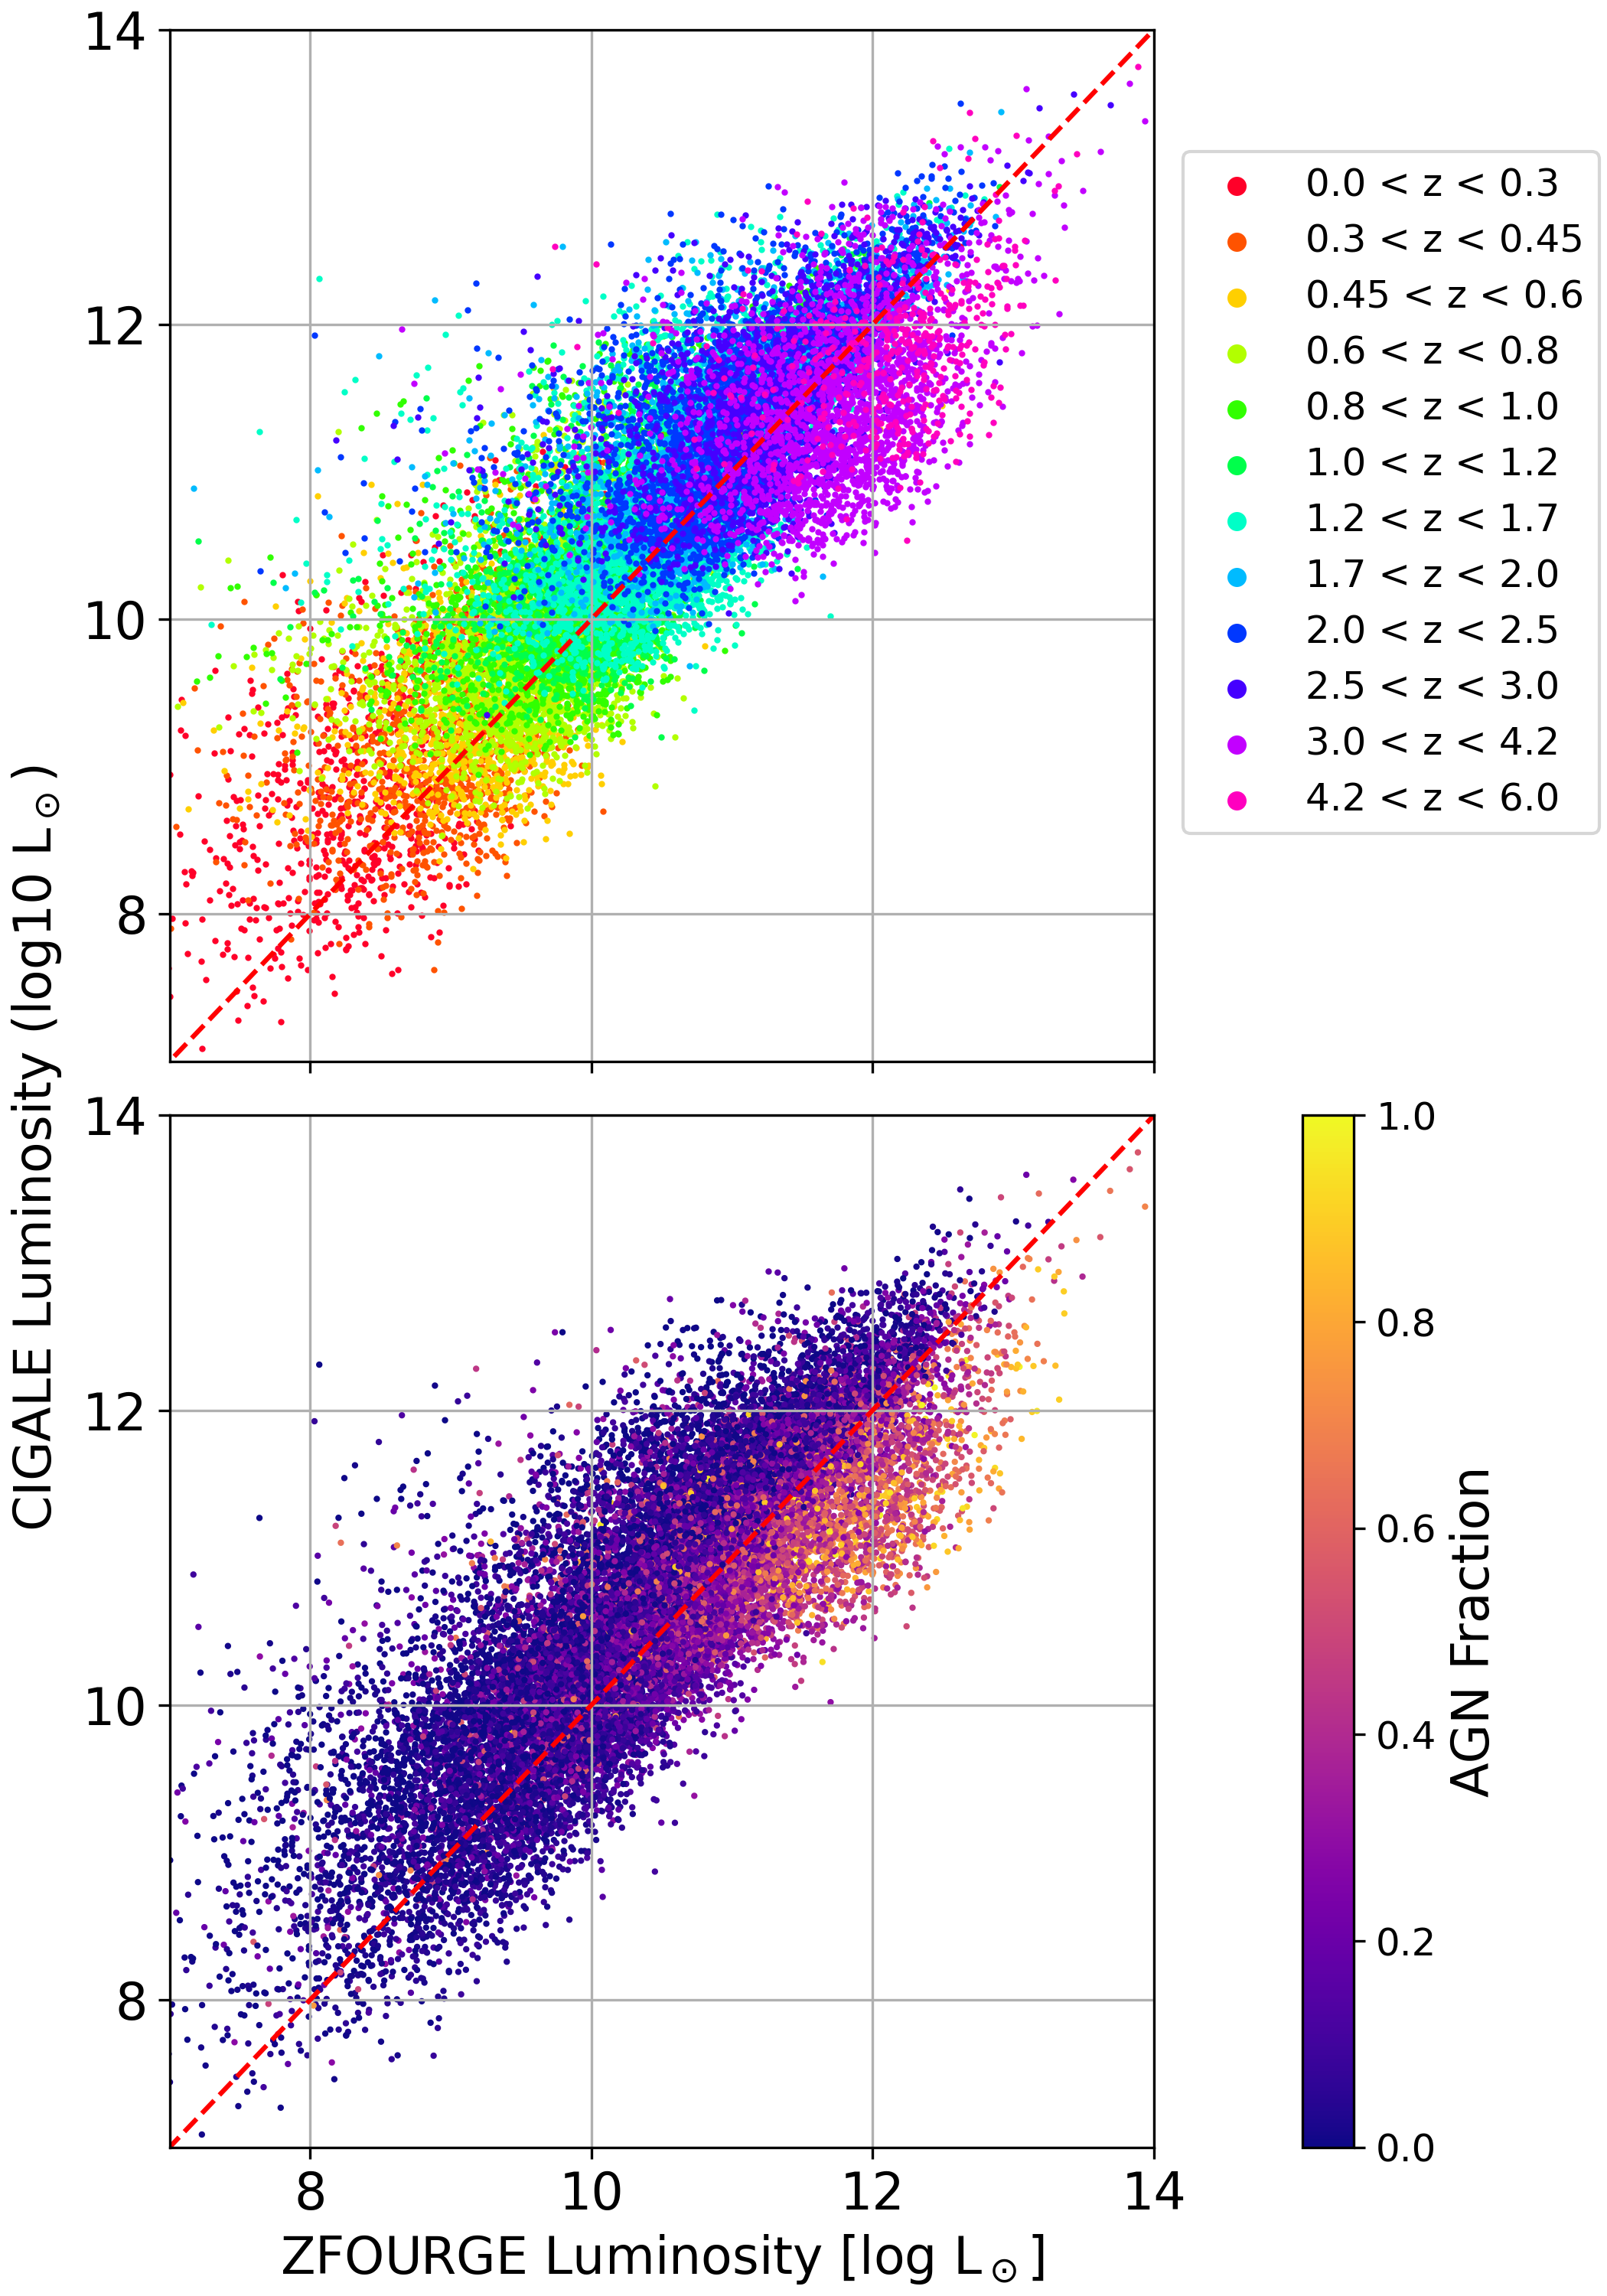
\includegraphics[width=0.9\textwidth]{Figures/LIR_vs_LIR.png}
    \caption{ZFOURGE total 8-1000$\mu$m IR luminosity compared to CIGALE total luminosity. Top: Sources coloured by redshift bin. Bottom: sources coloured by AGN fraction ($\mathcal{F}_{AGN}$). AGN fraction increases with redshift. At $z \geq 3$, the average AGN fraction is greater than 30\%.}
    \label{Fig: LIR vs LIR}
\end{figure}

\subsection{Robustness Tests with Mock Analysis} \label{Sec: Mock_Analysis}
To ensure the reliability of the decomposition process, particularly for faint AGN, we performed a series of robustness tests using CIGALE's built-in mock analysis. These tests evaluate the software's ability to accurately decompose AGN and SF contributions across various redshifts and luminosities, specifically focusing on galaxies with low IR luminosities.  The parameters were selected to balance physical realism, comparability with existing literature, and model performance across the redshift range. We also accounted for practical considerations such as degeneracy minimisation and reasonable processing time, which required adopting an approach with moderate resolution across select key parameters. By comparing the input and recovered AGN luminosities from the analysis, we confirmed that our parameter space and methodology are robust, particularly in detecting faint AGN. The mock analysis demonstrated that AGN luminosity was reliably constrained, with Pearson correlation coefficients (PCCs) ranging from 0.969 to 0.973 across all fields. Most sources lay within 0.5 dex of the 1-to-1 line, with mean residuals between $-0.02$ and $0.04$ dex, confirming the robustness of AGN luminosity recovery. These results indicate that our method effectively minimises bias against faint AGN, which are often difficult to detect in traditional analyses. Although the PCC values confirm reliable AGN recovery, potential systematics—such as AGN contamination of SF templates or the degeneracy in AGN/SF contributions—should be considered.

\subsection{Reliability of LIR Estimates Without FIR Constraints} \label{Sec: FIR Constraints}
ZFOURGE provides deep photometric coverage from the UV through near- and mid-infrared, but coverage at far-infrared (FIR) wavelengths, particularly at 160$\mu m$, is limited (Refer to Section \ref{Sec: CIGALE_Parameters}). Herschel PACS photometry is available for only a subset of sources in the CDFS field. To assess how this limitation affects our ability to recover LIR we performed a targeted mock-based validation using CIGALE.

We selected all galaxies with redshift $z > 2.5$ (a total of 6,940 sources) and compared their estimated $L_{IR}$ to the corresponding mock-recovered values provided by CIGALE. This test does not impose a MIPS SNR cut, ensuring that it captures the uncertainty across the full range of constraints available. Restricting the comparison to galaxies within the range $\log_{10}(L_{IR} [W]) \in [34, 40]$, we find:

\begin{itemize}
    \item Mean $\Delta \log L_{IR}$ = 0.004 dex (no systematic bias),
    \item Standard deviation = 0.27 dex,
    \item Normalized median absolute deviation (NMAD) = 0.14 dex
    \item ~19\% of sources show deviations greater than 0.3 dex.
\end{itemize}

These results indicate that CIGALE can recover IR luminosities with quantified and stable accuracy even for high-z sources lacking strong FIR constraints. This provides a quantitative bound on the uncertainty in $L_{IR}$ used throughout the luminosity function analysis. We add an additional error of 0.27 dex in luminosity to all sources at all redshifts and propagate this uncertainty to the luminosity function and beyond.

For a more comprehensive description of the SED decomposition methodology, see \cite{cowley_decoupled_2018}. Additionally, refer to the CIGALE software paper \citep{boquien_cigale_2019} for detailed information on its decomposition process and parameter optimisation techniques. 